% Text:              X
% Citations:         X
% Revision:          X
% Final Revision:    X
\chapter{Implementation}
The tool has now been used in a practical example to give an idea of how it is used to enhance the development experience.
This chapter will go into the design decisions and implementation details to make each part and feature of the tool function, as well as,
explain what the tool consists of and how the components work together to create the finished product.

The specifics of the code will be omitted, but the general control flow of each part of the tool will be explained.

\section{Overview of the Components}
The tool essentially consists of four components: The VS Code extension, the Svelte user interface, the Java program, and the NodeJS utility program.
The Java program is used to run the Jolie parser, which is also written in Java, and that will gather all information from the Jolie code needed by the visualization tool.

The Svelte user interface is the component which takes in the user input and renders the services, ports and connections.
In order for the UI to get the relevant data from the Jolie code, the VS Code extension invokes the NodeJS utility program, with the correct parameters, which invokes the Java program.
The NodeJS program listens for the output of the Java program,
meaning that the NodeJS program functions as a wrapper for the Java tool so the VS Code extension does not have to invoke the Java tool directly,
and sends the data to the VS Code extension, which sends the data to the Svelte UI.

Figure \ref*{figure:init_tool_sequence} shows the process of initializing the tool in VS Code, which is done using the \textit{visualize} command in VS Code.

\clearpage
\section{Data Representation}

\begin{figure}[h!]
    \center
    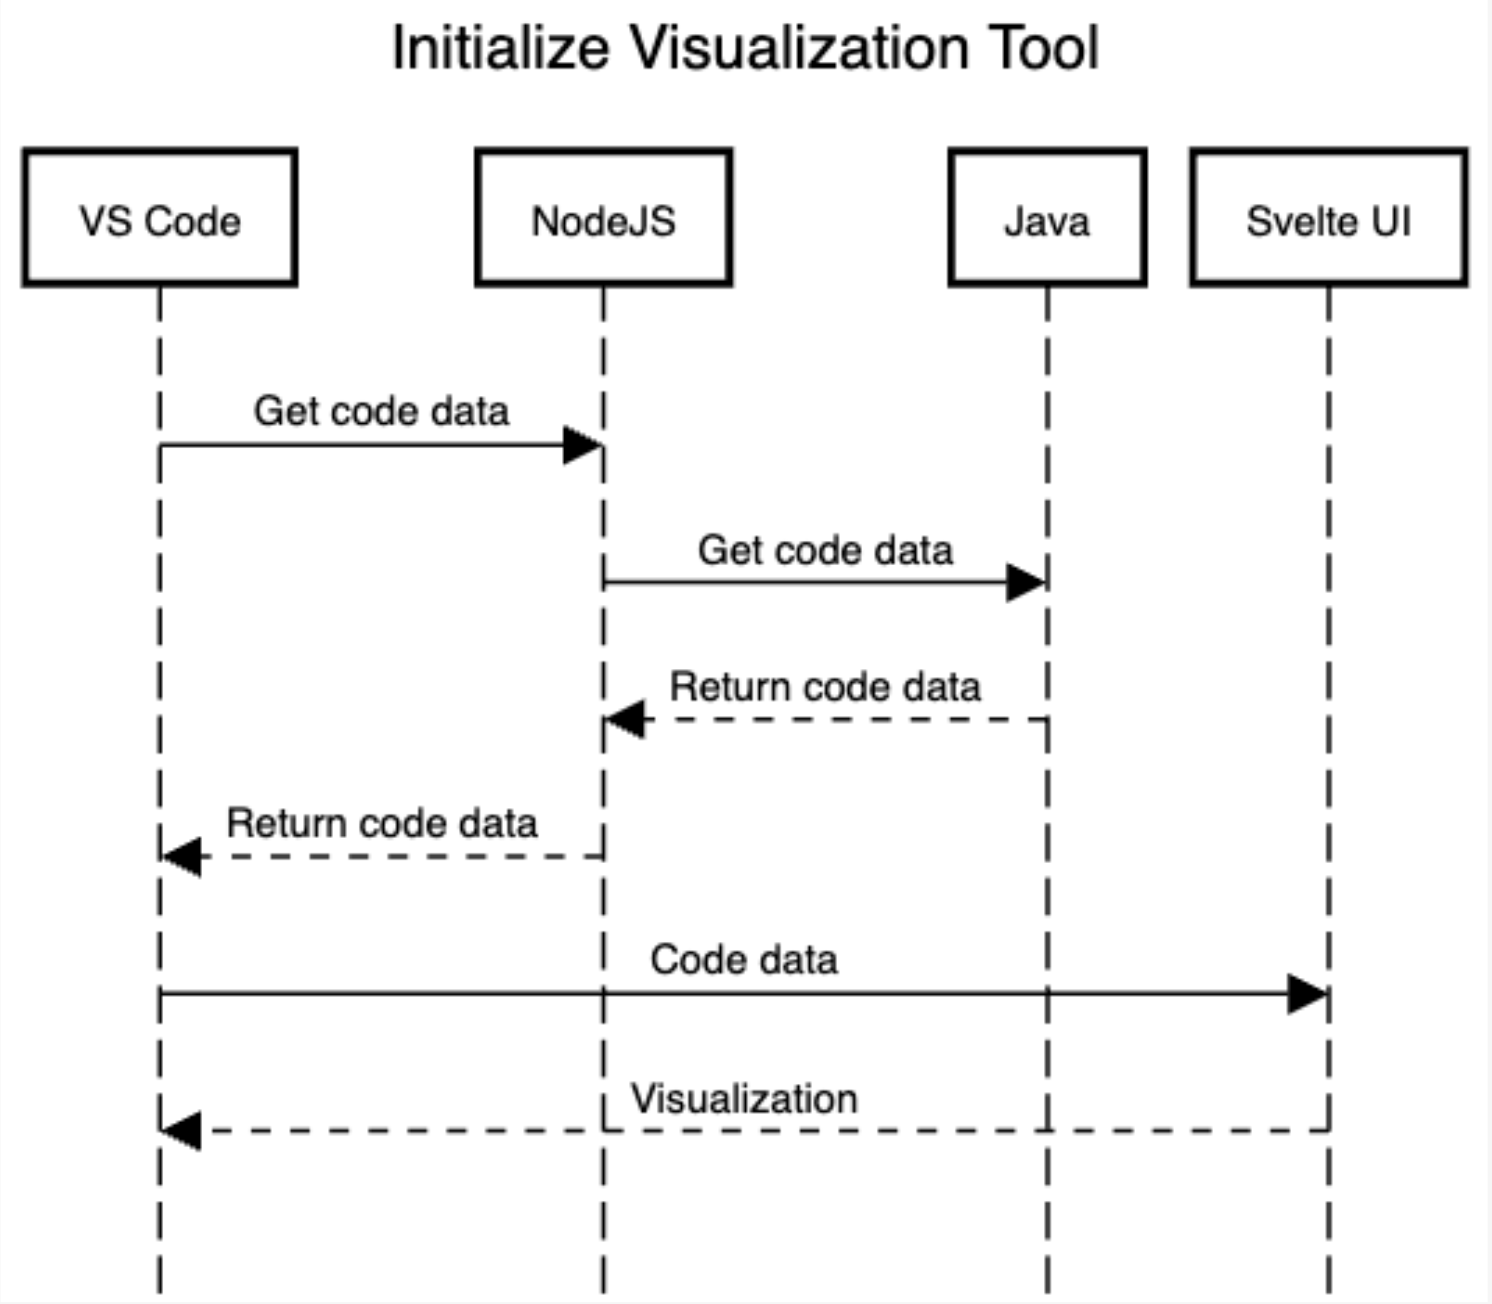
\includegraphics[width=0.70\textwidth]{figures/init_tool_sequence.png}
    \caption{A sequence diagram showing the sequence of requests and invocations between the four components that the tool consists of. The VS Code extension invokes the utility program using NodeJS which will handle running the Java program with the correct parameters, and afterwards, the VS Code extension sends that data to the Svelte UI which will visualize it in VS Code.}
    \label{figure:init_tool_sequence}
\end{figure}

The data which the Java program will output is consistent through all
four components of the tool. The chosen data format is JSON data because it is easy to parse in TypeScript, which all components consist of except for the Java program.
The data needed for the tool is a list of interfaces, a list of types and the list of services.

\subsection{Interfaces \& Types}
Each interface in the list of interfaces has a name, identifier, file path, and two lists of operations.
One of the lists contains all one-way operations, and the other contains all request-response operations.
The request-response operations consist of the operation name, the request type name-file path pair and the response type name-file path pair, and for one-way operations it is similar but with the response type omitted.
Having the type name and file path pair and a separate type object list instead of the type object directly in the specific interface object is a design decision made at the very start of the development process.
Each interface could have a list of types which will save computation when the user clicks on the type in the sidebar and the type is displayed because only the interface's list of types needs to be searched for the correct type.
This, however, has the drawback of a lot of duplication, only if all interfaces in the system use a unique set of types can this issue be avoided.
This is why a global list of types is used. The interfaces then reference what types are used for operation and the global list of types can be used when using the sidebar to view interfaces and types, and by
using the Jolie language constraint of no duplicate type names in the same OL file, the file path and type name are enough to find the correct type when searching for it.

The list of types, as mentioned, contains all types used by all interfaces in the architecture.
Each type object in the list represents the information about a type in the code, this includes the name of the type, the file in which the type is defined, the root type, subtypes which is a list of types as well, and cardinality of the type in case of this being defined.
If the type is a \textit{choice type}, the two choices are also represented in the type object as strings which reference other types in the global list.\footnote{Types in Jolie - \url{https://docs.jolie-lang.org/v1.10.x/language-tools-and-standard-library/basics/data-types/index.html}}
Types from \textit{interface extenders} are also added to this list.

\subsection{Services \& Networks}
The last list in the global JSON is the list of services. The list of services is also used to infer how the networks are set up and which services reside in each network.
This approach draws inspiration from how bigraphs are used to model software architecture. Bigraphs are a type of graph consisting of two sub-graph components. The link graph and the place graph. The link graph models the connection between nodes in the system while the place graph models the topology.
The nodes in the system of the bigraph can be directly mapped to Jolie services. Bigraphs also model ports which are a component of Jolie services as well.
The data representation used for the tool draws the most inspiration from the place graph since the link graph is inferred by the locations and protocols of the ports in Jolie.
A place graph models the topology and the networks, which are called \textit{roots} in bigraph terminology, and also embeddings, which are called \textit{nestings}.
The bigraph inspiration is taken from \textit{The Space and Motion of Communicating Agents} by Robin Milner \cite{BigraphBook}, where bigraphs are formally introduced and explained but are not necessary for this use-case.

The place graph component can be seen as a list of trees where the root is the network and contains all top-level services as immediate children and embeddings of the top-level services are the children of those services.
This fits well with how a Jolie system can be modelled, so the list of services in the global JSON is essentially a place graph or a list of trees where each node is a service in the system.
Each root in the list of trees is a network. In the sense of JSON, the network is a list of services since it can have any number of children, and the \textit{embeddings} list of each service is also a list of services.

The services in the JSON also need to contain all other information which is used by the tool.
This includes the input and output ports, execution target, name, identifier, and file path but also the information specified in the architecture file, which is container name, volumes, parameters etc.

\clearpage
\subsection{Architectural Programming}
The architectural programming features in Jolie also need to be represented in the data to visualize it in the tool's UI.
This includes couriers, collections, aggregations, and redirections. All of these aspects are created at the Jolie port level in the code, so the information is also represented in the ports of the JSON.

Aggregations in the JSON are represented by the name of the output port to aggregate to, optionally the aggregate can have an interface extender and which be defined here.
Collections are essentially a list of aggregations, so collections are also represented in the aggregates as a list of names of the output ports, and because multiple output ports of one service cannot have identical names, this will not create ambiguity.

Couriers are defined in Jolie based on an input port with aggregation, so the port also represents the couriers of that port.
The couriers in the JSON have lists of operation names and interface names which the courier will act upon. This is both for request-response and one-way operations. The names refer to the operations and interfaces in the system.

Redirections for an input port are a list of pairs of resource and output port names. This represents how a resource is redirected to an output port.
However, since the resource of the redirect is defined using the location of the output port, the output port will not be connected correctly unless the resource part of the string is removed, so the resource part of the location, namely,
the part after \texttt{/!/} is removed and placed in a separate field in the JSON for the output ports.

\subsection{Prototype Data}
The data used to create the prototype is also represented in JSON and is split into two parts, the Docker-Compose YAML file content and the service folders which contains the Jolie files, dependencies, and Dockerfile.
The Docker-Compose file content is simply a string, which will be written to the file. The build folders are used to generate this string, but this will be explained more in detail in a later section.
The services folders, which are called build folders internally, are an array of objects that each represent a folder to be created when generating the prototype.
The build folders have to represent what a Docker image will contain, so each folder can be seen as a Docker image. This has to be independent of the Jolie code since two identical services can have different parameters or runtime arguments.

Each build folder contains a list of files which will be added to the folder itself, but also a list of files which will be added to the shared resource folder.
Information such as runtime arguments, exposed Docker ports, and the service name is also added to the build folder JSON because the Dockerfile needs this information when it is being generated.

\section{NodeJS Utility Program}
% why it is created and how it works
The NodeJS utility program functions as a wrapper for the Java program. It is created so the VS Code application does not have to execute the Java program directly and also if the tool should be extended to other code editors or run in the browser, this functionality should not be implemented in the VS Code extension.
The NodeJS program also makes sure to return errors if a parsing error occurs or if Jolie is not installed correctly.

This part of the tool consists of three parts, the data fetching part which executes the Java program and checks for errors, the server part which allows the developer to visualize their program's architecture directly in the browser but without the code refactoring functionality, and
prototyping which is identical to the functionality in the VS Code extension, but this can be used if the user of the tool installs only this part of the tool without the VS Code extension.
The server uses the express framework\footnote{Express Framework - \url{https://expressjs.com/}} to open an endpoint to get the JSON data and also serve the webpage as static assets on localhost.

\section{Java Program}
% how the data is fetched in the Java tool
The Java program is used to gather the required information from the Jolie code. The Jolie parser is written in Java and therefore the Java program here uses the parser directly to get the abstract syntax tree nodes and create the JSON objects.

The Java program has two types of outputs which is used by the tool. The JSON representation of the entire system and the information used by the prototyping functionality. Both functionalities of the Java program require the whole system to be parsed using the Jolie parser.
Firstly, the tool creates the networks by parsing the architecture JSON file and making an internal representation of what it contains. The networks contain a map of top-level services mapped to a \texttt{ServiceNode} which is the abstract syntax tree (AST) node of a service from the Jolie parser. The top-level service is a representation of a Jolie service in the architecture file, as seen in appendix \ref*{appen:architecture-file-structure}.
The Java program uses a lightweight JSON library, \textit{json-simple}, to parse files and create JSON objects\footnote{JSON-simple - \url{https://code.google.com/archive/p/json-simple/}}.
To get the ServiceNode AST node from the parser, the Jolie parser is invoked using its module parsing method. This returns the whole AST of a file, called a \textit{program}. All ServiceNodes are then captured and added to the network's map object.

When the networks have been created, depending on if the program should send visualization data or prototyping data, all the necessary information about the services, ports, etc. is created.
\subsection{Parsing the Jolie System}
A system inspector has been created in order to parse the networks.
The system inspector uses the created list of networks containing the top-level services and ServiceNodes.
The inspector goes through each network's map object and creates a service object which is an internal representation of the services used by the tool.
It creates the services by looking at all the child nodes of the ServiceNode AST node in a loop and using type comparison to check what child node is being looked at and how to parse the information correctly.
Relevant child nodes for a service are: \textit{ExecutionInfo}, \textit{CourierDefinitionNodes}, \textit{EmbedServiceNodes}, \textit{InputPortInfo}, and \textit{OutputPortInfo} nodes.

Service objects can also have a list of services which are considered embeddings. When looping through the AST nodes of a service, embedded service nodes will be used to create services, which are added to the parent's list of services instead of the global list of services.
This will enforce the place graph structure of services mentioned in the data representation section.

The most complex of the child nodes are the two types of port nodes. Input and output ports also have an internal representation in the Java program which keeps track of all the necessary information about the ports used by the tool.
Ports have to contain information about the location, protocol, name, interfaces and operations.
When the ports are being created, the interfaces which are used by the ports will also be created. These interfaces are also represented internally and will store information about the operations.
The operations are also parsed using type comparison, since two types of operation declaration AST nodes exist in Jolie, namely, request-response and one-way.
The interfaces are added to a global object \textit{JolieSystem} which has information about all parsed services and interfaces.

For input ports specifically, information about aggregates, couriers and redirects is also stored. Redirects can be seen as a mapping where a resource is mapped to a port name. This is how the Jolie parser represents redirects as well, so this is simply copied over to the tool's representation.
Aggregates are simply a name of an output port but can contain collections and interface extenders, however, Jolie's internal representation of aggregates contains this information so the interface extender just has to be created to match the tool's representation of interfaces, and collections are a list of output ports which will be copied directly.

When the interfaces are created the types used in the operations are also parsed and created in an internal representation.
This representation stores information about the root type, cardinality, subtypes, etc.
The types in Jolie can also be three different AST node types, namely definition links, inline definitions and choice definitions. Type comparison is also used here to parse the type correctly depending on the AST node type.
Types are, similarly to interfaces, added to the system's global list of types.

Each building block of a Jolie service has an internal representation in the Java program, and all of them have a \texttt{toJSON} method which takes all information stored in the objects and creates a JSON object.
When the tool invokes the Java program to get the JSON data, the \texttt{getJSON} method is invoked on the global JolieSystem object which cascades and invokes the getJSON method for all internal objects which also carcades to its internal objects.
This will result in a JSON object which resembles the data representation discussed in the previous section, and this JSON can be used by the other components of the tool.

\subsection{Generating the Prototype Data}
The Java program also creates data for making the prototype. This includes the content of the Docker-Compose YAML file and the information needed for creating the service folders and the resource folder.
After the whole system has been parsed and a JolieSystem is created, the system will be given as a parameter to a \textit{build} object which will handle the logic for creating the JSON data.
The builder will first create the service folders using the services in the networks from the JolieSystem object. Duplicate build folders will be checked for at this stage, which is done to make sure that duplicate images will not be generated when using Docker-Compose.
However, as mentioned in a previous section, two identical services can be two different images if the runtime arguments are different, which is also handled here.

After the build folders have been created as internal objects, they are parsed onto another object which builds the Docker-Compose YAML string. The JolieSystem is also used here to create the networks in the Docker-Compose file.
The Docker-Compose builder also has some internal representation of what a service is, since two services in Docker-Compose can use the same image but have different deployment properties, which means that they should be created as separate services in Docker-Compose, but they will not have two different service folders.
The Docker-Compose builder uses a string builder to create the YAML file content. It goes through all services and creates an internal \textit{compose service} and like with the service folders, composes duplicates and counts replicas.

The networks are also created in the Docker-Compose YAML, which can have another semantic meaning from the networks defined in the architecture file.
In Docker-Compose networks are used to restrict services connecting, which is not a problem with a system created in Jolie, so to have the Docker-Compose networks work similarly to how networks in the tool work, each service in Docker-Compose is set to be a part of
its network, as specified in the architecture file, but also all other networks that the service has a port connecting to.\footnote{Networks in Docker-Compose - \url{https://docs.docker.com/compose/networking/}}

\section{Visualization User Interface}
After the JSON data has been created using the Java program, it needs to be rendered in a user interface, which can handle user input as well.
There are two aspects of these components, firstly, how to create a reactive user interface which can handle user input and handle updates based on how the user interacts with the tool. Secondly, how the components of the architecture are rendered efficiently and how they should be laid out to make the architecture readable and manageable.

\subsection{User Interface}
The tool's user interface is essentially a static webpage where the JSON data is loaded when the site is initialized.
The UI uses CSS for styling and JavaScript for the logic, like most standard websites.

However, creating a very feature-heavy reactive user interface in standard CSS and JavaScript is almost impossible in a reasonable amount of time.
The first improvement to the development of the UI was to replace JavaScript with TypeScript (TS).
TS is a compiled and strongly typed programming language, created by Microsoft, which is a superset of JavaScript. It compiles directly to JavaScript which makes it usable by the UI webpage.
Some of the benefits of using TS include type checking, self-documenting code, interfaces, and generally enhanced productivity.\footnote{TypeScript - \url{https://www.typescriptlang.org/}}
% todo more about TS??

Writing standard CSS can also be a very tedious process, so to enhance the development experience TailwindCSS, or just Tailwind, is used.
Tailwind is a CSS framework which aims to move CSS to the HTML components. CSS properties are defined in the class attributes of the HTML components where readable class names have been defined meaning that any combination of these classes can be used to style components.
Tailwind also defines a design system which a developer can use to enforce a standard when it comes to the design of the UI, and with tools like \textit{postcss} and \textit{autoprefixer} the build size of the utility CSS components will be kept at a minimum.\footnote{TailwindCSS - \url{https://tailwindcss.com/}}

The last overall part of the UI is the actual content of the webpage. All services, ports and edges between ports are rendered using SVG components.
Different SVG\footnote{SVG Elements - \url{https://developer.mozilla.org/en-US/docs/Web/SVG}} elements are used for different parts of the UI. Polygons are used to render service shapes, rectangles are used to render ports and paths are used to render edges between ports.
SVG elements in HTML are easy to manipulate in TS, so when the JSON data is loaded in, the correct HTML components are created and then TS is used to create the SVG data for each component so they get the desired shape and size.
To help with the manipulation of SVG elements in TS, a library is used called \textit{D3.js}.\footnote{D3.JS - \url{https://d3js.org/}} D3 has a long list of features to help visualize data using SVGs, however, the only functionality used for this tool is
the ability to select SVG components and apply attributes, event handlers, and stylings.

\subsection{UI Framework}
% svelte
To facilitate the reactivity needed for the UI when the user starts manipulating the architecture, a UI framework called \textit{Svelte}\footnote{Svelte - \url{https://svelte.dev/}} is used.
Svelte is a framework used to create reactive web interfaces similar to React, Angular, and Vue. The benefit of using Svelte instead of any of the other frameworks mentioned is that Svelte compiles into highly efficient JavaScript,
whereas most of the other frameworks ship some sort of DOM manipulation engine alongside the code. Svelte is the chosen framework because it must run in VS Code which runs in Electron, and the speed is a factor in this case.

\subsection{Rendering \& Layout}
% first version of the tool

% elk
In the first version of the tool the service shapes had a direction, meaning that all input ports were on the same side of the service shape, this meant that the layout of the services was easier to solve.
At first, the layout algorithm used for the services was a naive horizontal layered algorithm where the services were given priority depending on how many input and output ports the service had.
Services with the highest priority will be rendered in the leftmost layer. Services with only input ports were considered the highest priority and services with only output ports will be rendered in the rightmost layer.
This solution only worked with services where all input ports where on the left side of the service and all output ports were on the right side of the service.

Services having a direction and all the same types of ports being placed on the same side do not work when larger architectures need to be visualized.

\section{Visual Studio Code Extension}
% how the vscode extension works
% vscode api
% webviews
% live reload
% code ranges and parsing context 
% live architecture update

\subsection{Code Refactoring}
% Editing properties of the services and ports using the sidebar we
\subsection{Embedding \& Disembedding}
% auto import
\subsection{The Aggregator Pattern}

\section{Prototyping}
% generating docker compose files
% getting dependencies
\subsection{Dependencies}
\clearpage